\documentclass[11pt, a4paper]{article}
\usepackage[a4paper, total={6.5 in,9in}]{geometry}
\usepackage[slovene]{babel}
\usepackage[utf8]{inputenc}
\usepackage[T1]{fontenc}
\usepackage{lmodern}
\usepackage{amsmath}
\usepackage{ amssymb }
\usepackage{amsfonts}
\usepackage{amsthm}
\usepackage{comment}
\usepackage{url}
\usepackage{gensymb}
\usepackage{subcaption}
\usepackage[pdftex]{graphicx}
\usepackage[section]{placeins}
\usepackage{mathtools}
\usepackage{float}
\usepackage{epstopdf}
\renewcommand{\vec}[1]{\mathbf{#1}}
\usepackage{hyperref}
\usepackage{wrapfig}

\pagestyle{plain}

\begin{document}

    \begin{center}
    {\LARGE\bfseries 10. Metropolisov algoritem\par}
    \vspace{1cm}
    
    {\Large Domača naloga pri predmetu Modelska analiza I\par}
    \vspace{0.2cm}
    {\normalsize Avtor: Matic Noč \par}
    \vspace{0.2cm}    
    {\normalsize 15.11.2017 \par}    

    
    \end{center}
\section{Uvod}
Obravnavamo algoritem Metropolis-Hasting, ki je prvotno namenjen aproksimaciji neke porazdelitve $P(\vec{x})$, ki jo ne moremo izračunati s pomočjo obratne vrednosti konvolucijske funkcije ali pa obdati porazdelitev približno porazdelitvijo, saj v več dimenzionalnih problemih pogosto ne znamo sploh opisati analtično. Take procese se da prikladno uporabiti v minimizacijskem problemu, kjer nam algoritem Metropolois-Hasting omogoča, da poleg sledenja verjetnostni porazdelitvi v smeri minimuma, skačemo iz lokalnih minimumov v druga območja s neko $verjetnostjo$ $sprejetja$, v ozadju pa tečejo Markovske verige, ki temeljijo na slučajnem procesu, ki je odvisen le od prejšnega procesa (ne pozna zgodovine) in tako lahko vsako novo stanje sistema vzamemo glede na verjetnost $predhodnega$ in $trenutnega$ stanja, ki pa jo pogosto aproksimiramo kar s funkcijo $f(\vec{x})$ ali pa boltzmanovo statistiko $e^{\frac{-E}{k_B T}}$, kjer je $E$ energija sistema.
\section{Metropolisov optimizacijski algortiem}
Imamo porazdelitev $P(\vec{x})$, iz katere želimo vzorčiti stanja $\vec{x}$. Ta stanja so lahko poljubno dimenzionalna, npr $N_a$ delcev, ki ima skupaj energijo $E = \sum_i W_{ki}$.  Potem stanje sistema $\vec{x}_i$ spremenimo s potezo (ponavadi le en del stanja x). Recimo, da obe stanji izžrebamo naključno s enako verjetnostjo. Recimo da želimo vzorčiti stanja iz Boltzmanove porazdelitve. Pri takšnem procesu se nam Markovski člen, ki velja za detaljno ravnovesje $\frac{P(\vec{x'} \rightarrow \vec{x})} {P(\vec{x} \rightarrow \vec{x'})}$, pretvori v 
\begin{equation}
\frac{e^{-\frac{f(\vec{x_{i+1}})}{k_B T}}}{e^{-\frac{f(\vec{x}}{k_B T}})} = e^{- \Delta f / k_B T} = \alpha 
\end{equation}
S tako verjetnostjo želimo sprejeti naše naslednje stanje $\vec{x_{i+1}}$. Verjetnost s katero bomo sprejeli naše stanje $\vec{x_{i+1}}$ dobimo iz minimuma
\begin{equation}
min ( 1, e^{- \Delta f / k_B T} ).
\end{equation}
Torej ko bo $\Delta f  < 0 $, vedno sprejmemo stanje, saj prehajamo v minimum funkcije, drugače pa sprejemo novo stanje s verjetnostjo $e^{- \Delta f / k_B T}$, kar v praksi simuliramo tako da naključno žrebamo $ u \in U(0,1)$ in nato primerjamo 
\begin{equation}
u \leqslant \alpha,
\end{equation}
potem stanje sprejemo. To lahko opravičimo s tem, da je naša verjetnost $e^{- \Delta f / k_B T} \in [0,1]$. Recimo da je $P = 0.7$. Pri enakomernem žrebu je verjetnost, da se žrebano število $u$ nahaja levo od $0.7$ ravno $70 \%$. 
\newline\newline
V naši verjetnosti za sprejetje nastopa tudi temperatura $T$, ki nam določa, kako močno bomo skakali po faznem prostoru. $T \rightarrow \infty$ nam bo sprejela vse slabše izide, $T \rightarrow 0$ pa nobenega. Torej, ko so stvari vroče lahko pregledamo fazni prostor, bolj ko hladimo manj dopustimo premikov iz danih minimumov. Če bomo ohlajali dovolj počasi, bomo sigurno padli v globalni minimum in se pomikali po njem navzdol. Take vrste algoritem se imenuje simulirano ohlajanje (ang. $simulated $ $annealing$, ki izvira iz ideje postopnega ohlajanja kovin za lepšo kristalno zgradbo.
\section{Molekularna verižnica}
Zanima nas kako se bodo postavili 17 členov in dva fiksna na robu, ki sestavljajo molekulo. Na voljo imajo 19 višinskih nivojev. Molekula strmi k čim nižji potencialni energiji, ki je zaradi ničle na vrhu enaka
\begin{equation}
E = \sum_i^N \alpha h_i < 0 
\end{equation}
seveda pa morajo biti členi molekule ne predolgi, zato moramo tudi odmike kaznovati s tem, da se energija veča, če je člen verige med sosednjima nivojema preveč raztegnjen, torej
\begin{equation}
E = \sum_i^N \alpha h_i  + \frac{1}{2} k \sum_i^N (h_{i+1} - h_i)^2
\end{equation}
Vzemimo  $k = 1$, kar nam bo olajšalo računanje spremembe energije.
V vsakem stanju $\vec{X_i}$ lahko izračunamo energijo stanja; \newline\textbf{Iščemo takšno stanje $X$, kjer bo energija sistema najmanjša}. \newline\newline
Če bi imeli veliko molekul bi bila energija sistema potratna za računanje, zato spremnijamo le del molekule s \textbf{potezami}. V primeru ko je poteza narejena le na enem členu molekule , lahko izračunamo spremembo energije kot
\begin{equation} 
\Delta E = E' - E = \alpha (h'_{i} - h_{i}) + \sum_{j \in [ i -1 , i +1]} \frac{1}{2} ((h'_i - h'_j)^2 - (h_i - h_j)^2)
\end{equation}
Če energijo sosedov razpišemo dobimo
\begin{equation}
\Delta E  = \alpha(h_i' -h_i) - h_{i-1} (h_i' - h_i) - h_{i+1} (h_i' - h_i) + h_i'^2 -h_i^2
\end{equation}
Če je $h_i \rightarrow h_i + \delta_i$, kjer je $\delta_i = \pm 1$, potem dobimo
\begin{equation}
\Delta E = \delta_i^2 - \delta_i ( h_{i+1} + h_{i-i} -2 h_i - \alpha)
\end{equation}
Če je $\delta_i = 1 $ vidimo ,da povečujemo potencialno energijo saj dobimo člen $+ \alpha$, če pa je $\delta_i = -1 $ pa zmanjšujemo potencialno energijo, saj nastopa člen $-\alpha$. Prožnostna energija pa je odvisna od pozicije sosednjih molekul $h_{i+1} $ in $ h_{i-1}$.
\subsection{Omejena verižica}
Poglejmo si oblike verižice v odvisnosti od temperature pri $n=10000$ iteracij, $k_B = 1$, $\alpha = 1$ in različnih temperaturah:
\begin{figure}[H]
\centering

  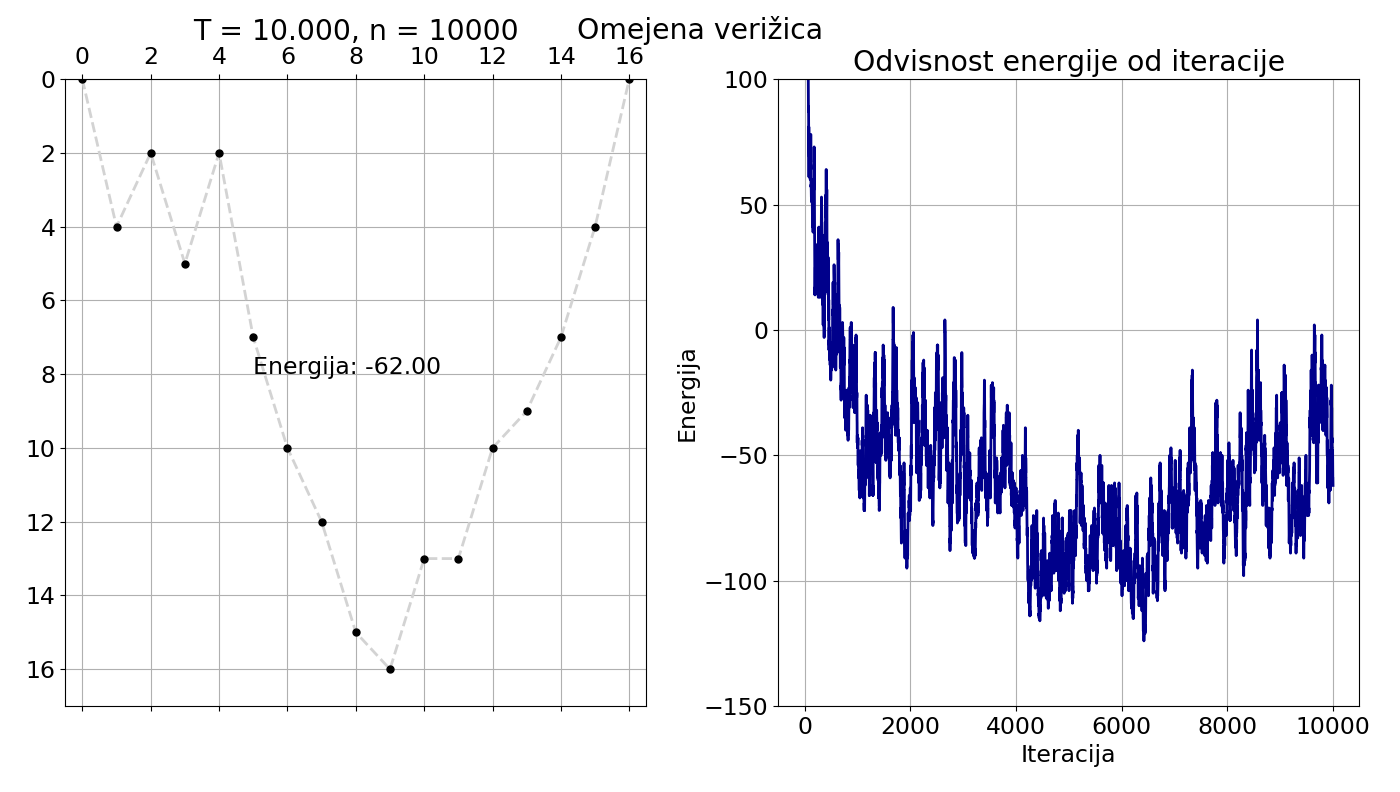
\includegraphics[width=16cm, height=4cm]{omejena_globina_T0_10.png}
 
\end{figure} 
\begin{figure}[H]
\centering

  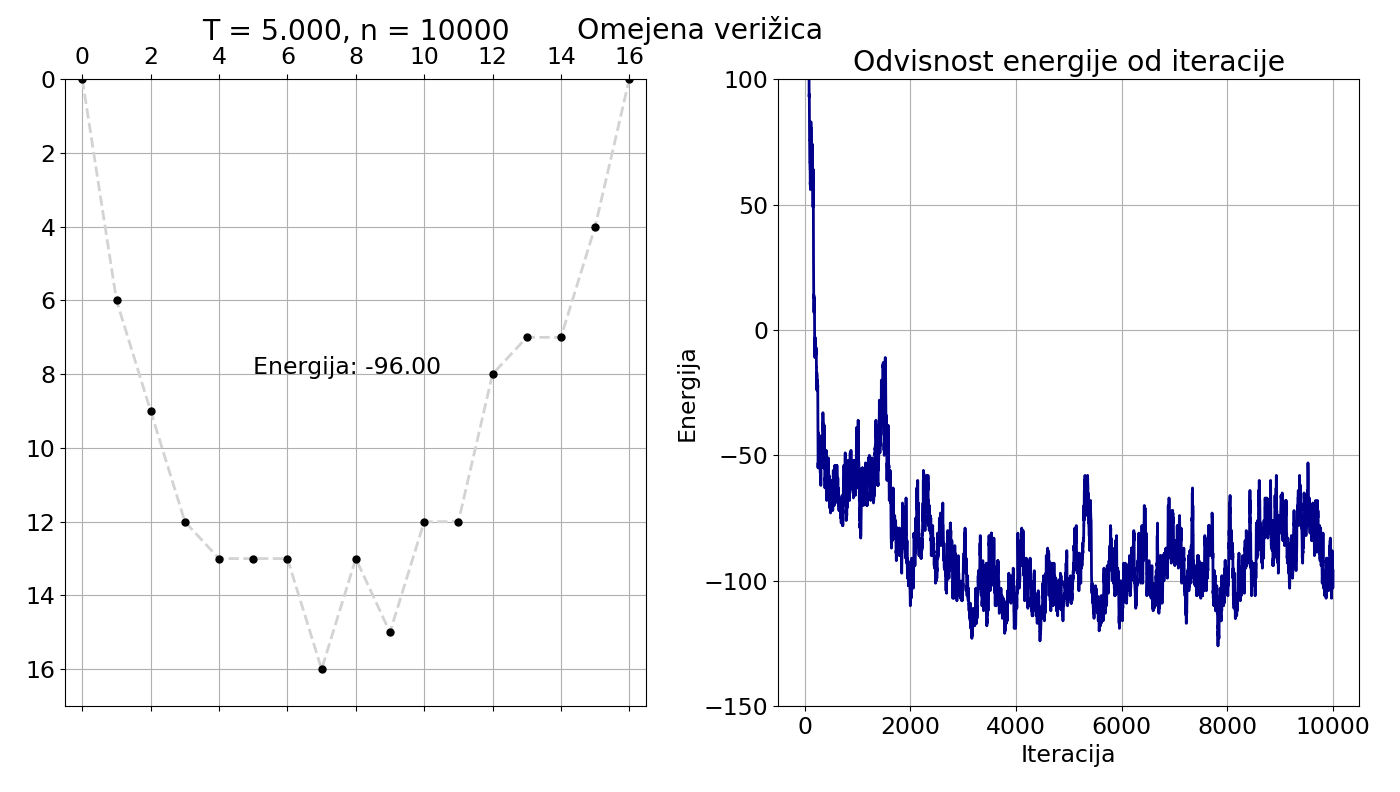
\includegraphics[width=16cm, height=4cm]{omejena_globina_T0_5.png}
 
\end{figure} 
\begin{figure}[H]
\centering

  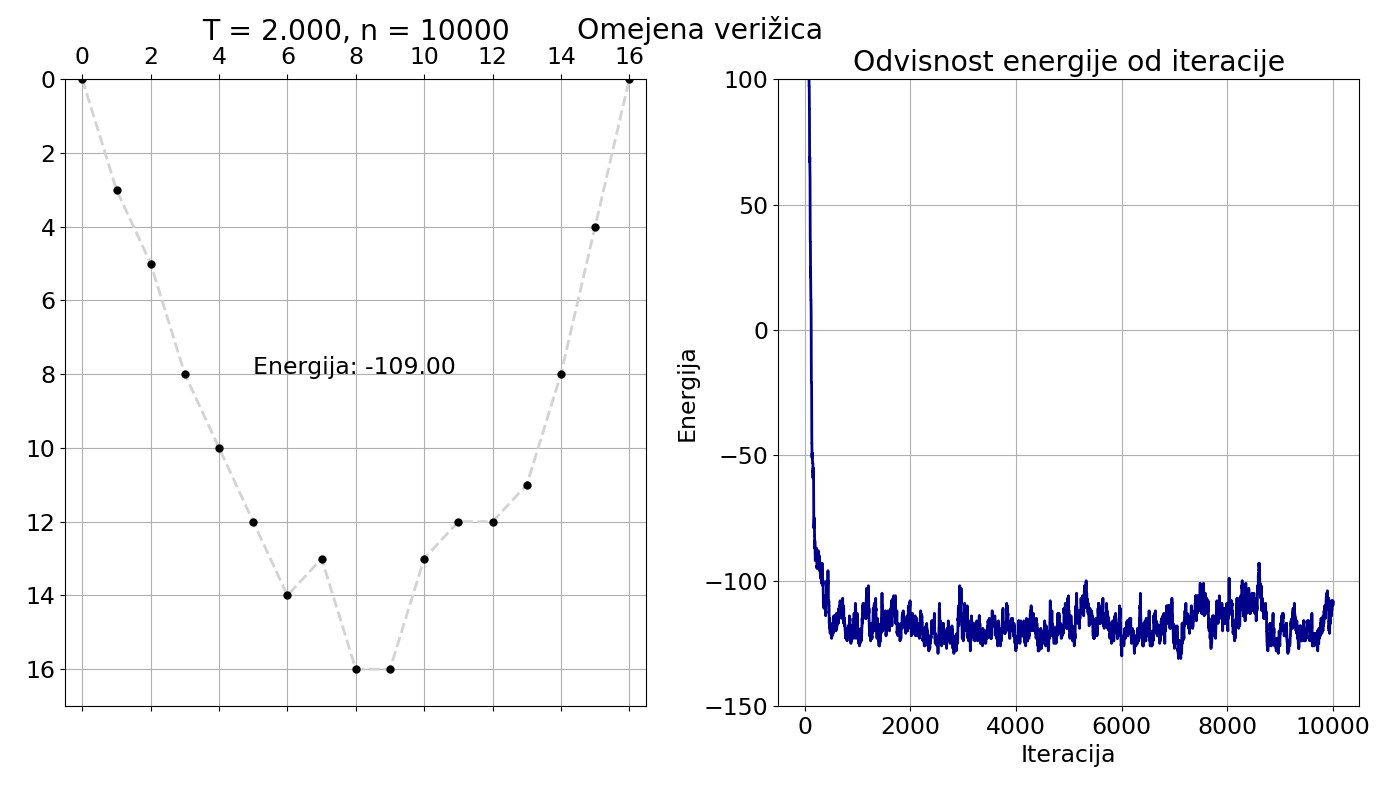
\includegraphics[width=16cm, height=4cm]{omejena_globina_T0_2.png}
 
\end{figure} 
\begin{figure}[H]

\centering
  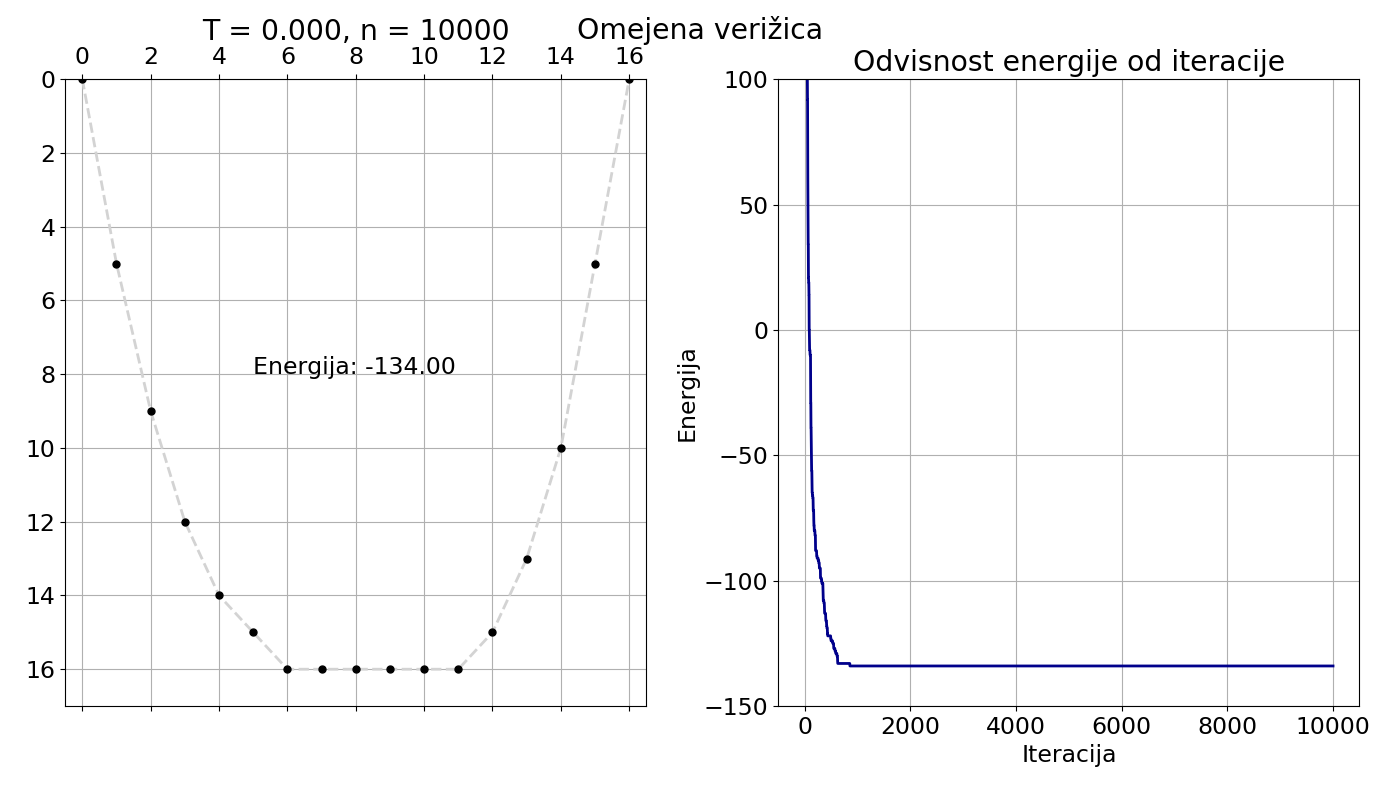
\includegraphics[width=16cm, height=4cm]{omejena_globina_T0_0.png}
 
\end{figure} 
Iz grafov lepo vidimo vpliv temperature na sistem. Ko je temperatura visoka, so dopuščene fluktuacije energije večje, zato lahko skačemo ven iz potencialnih minimumov. Pri temperaturi 0 ima verižica obliko, kot bi jo imela prava verižica, ki se pogrezne zaradi lastne teže, vendar pa tla ne dopuščajo da se ugrezne do konca. Ko imamo temperaturo 0, sprejmemo le dobre poteze, zato lahko ugotovimo, da ima problem verižice \textbf{lokalni} minimum enak \textbf{globalnemu}.
\subsection{Neomejena verižica}  
\begin{figure}[H]
\centering

  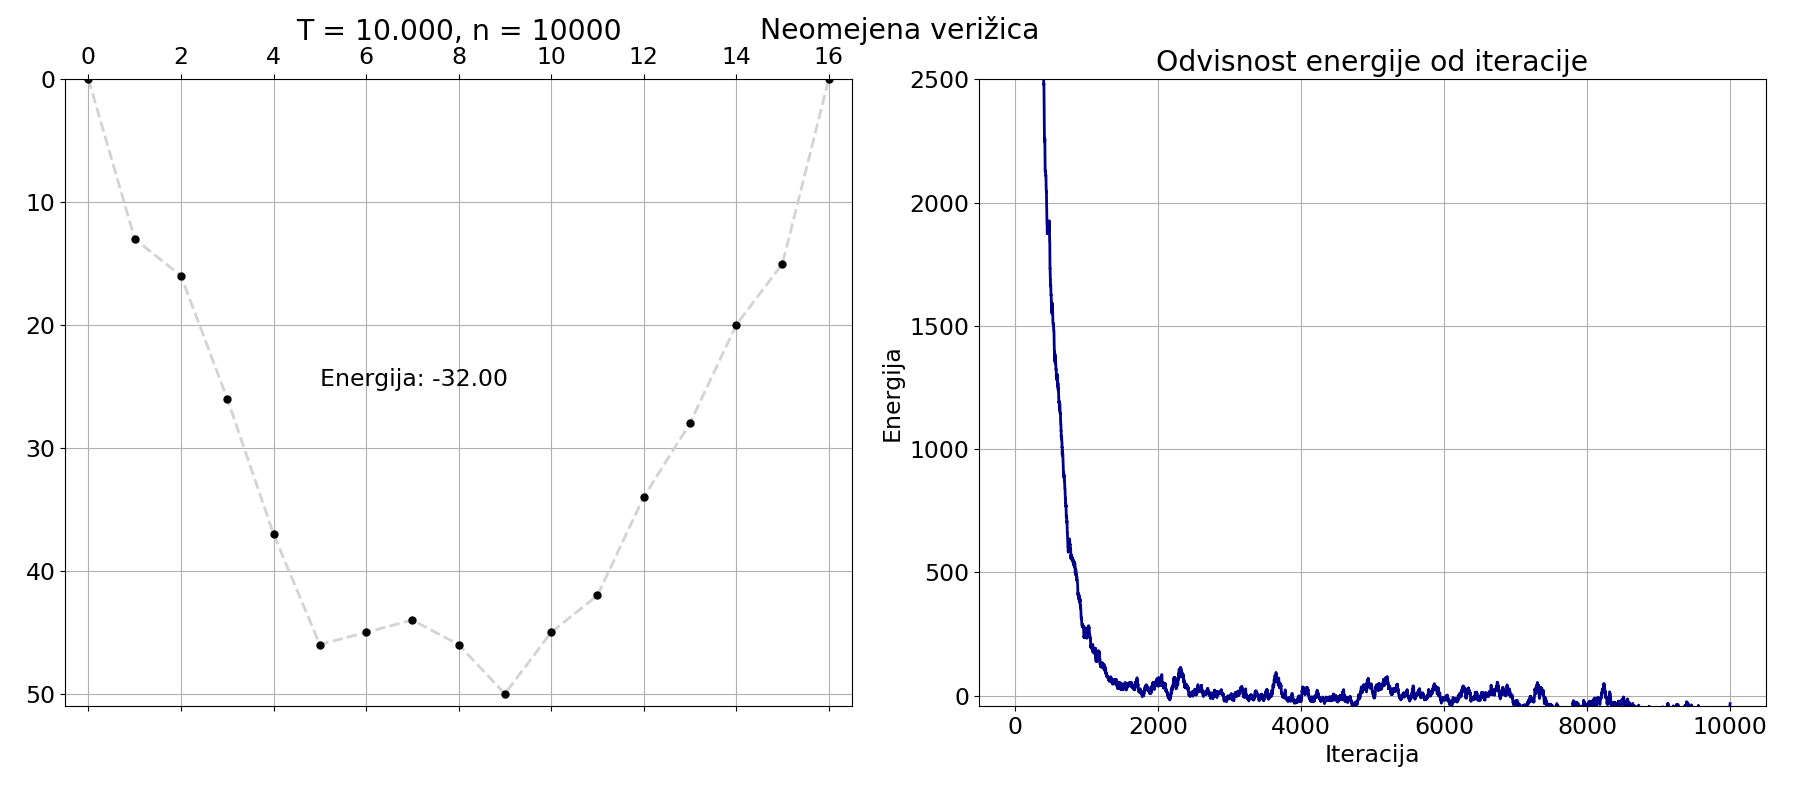
\includegraphics[width=16cm, height=4cm]{neomejena_globina_T0_10.png}
 
\end{figure} 
\begin{figure}[H]
\centering

  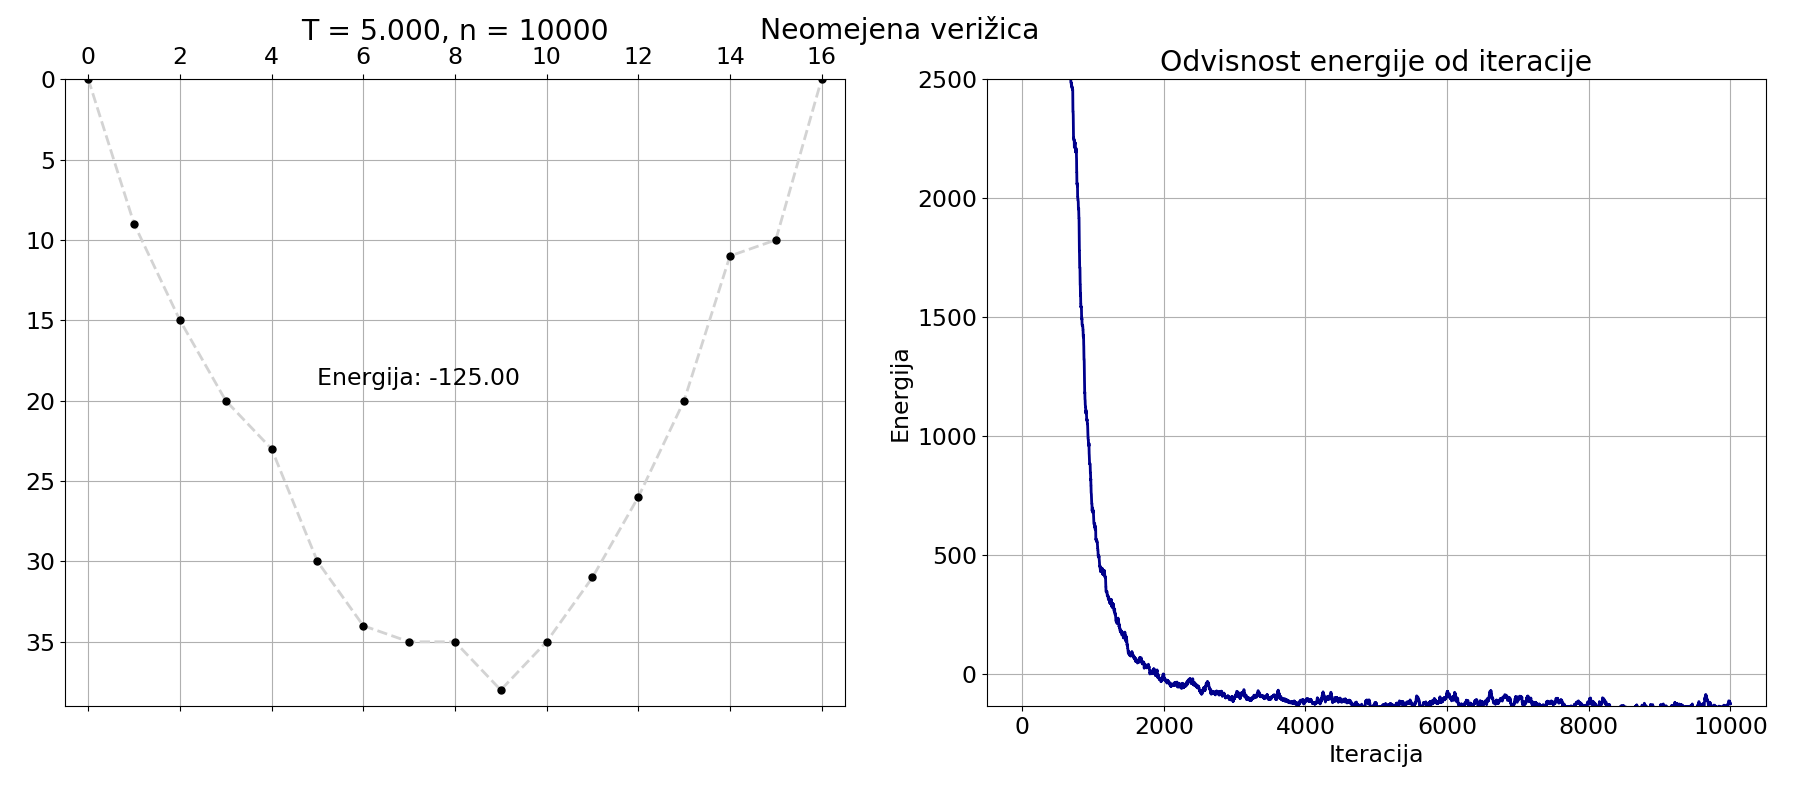
\includegraphics[width=16cm, height=4cm]{neomejena_globina_T0_5.png}
 
\end{figure} 
\begin{figure}[H]
\centering

  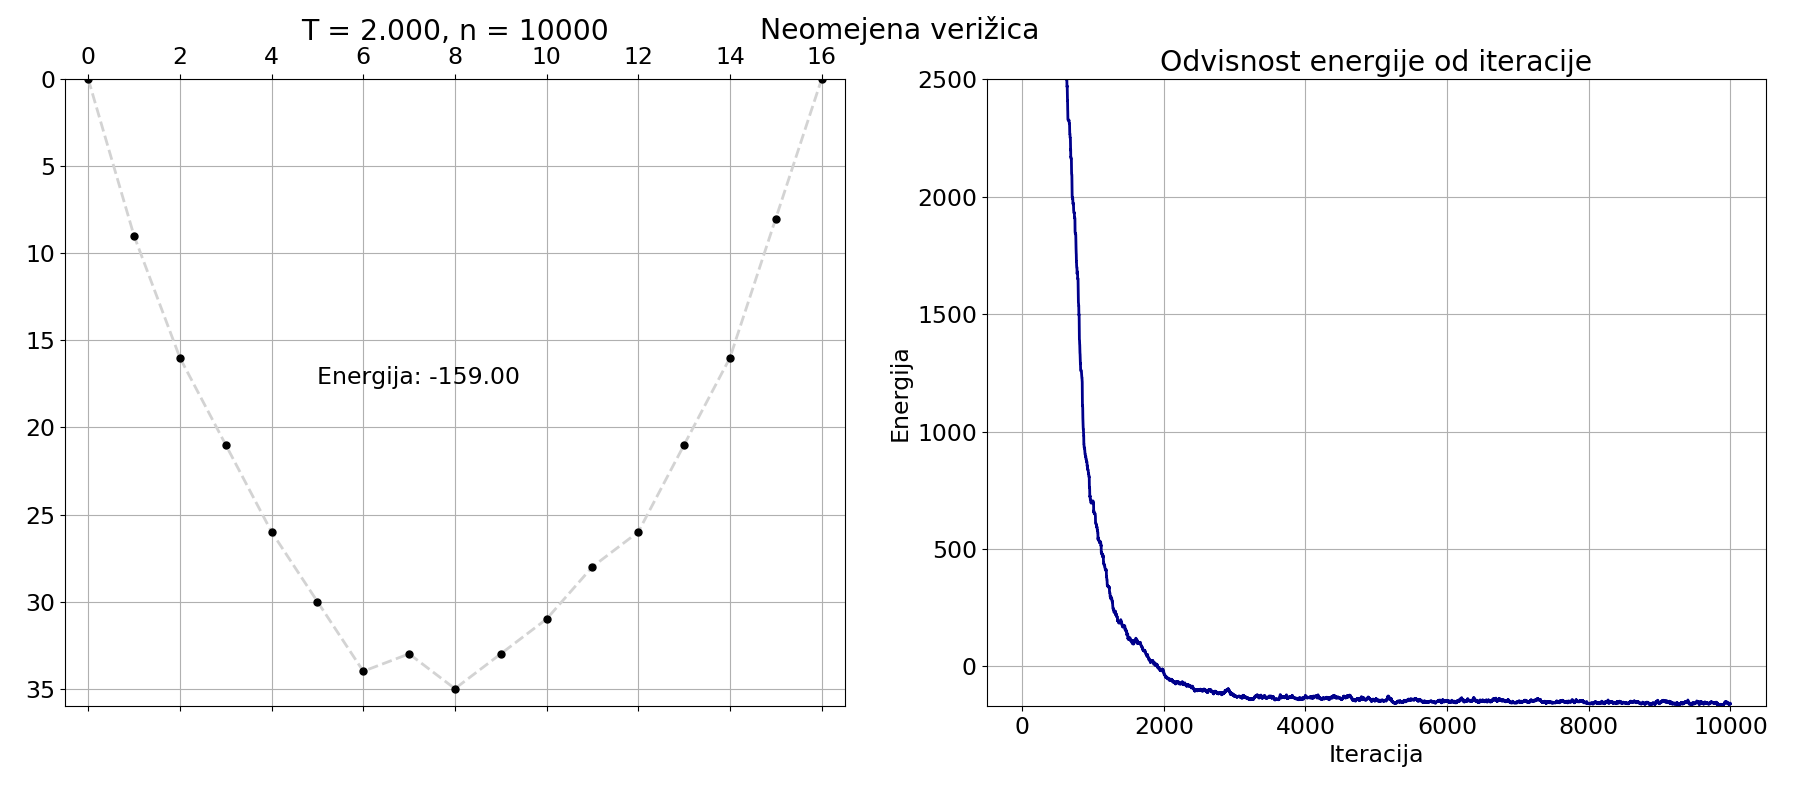
\includegraphics[width=16cm, height=4cm]{neomejena_globina_T0_2.png}
 
\end{figure} 
\begin{figure}[H]

\centering
  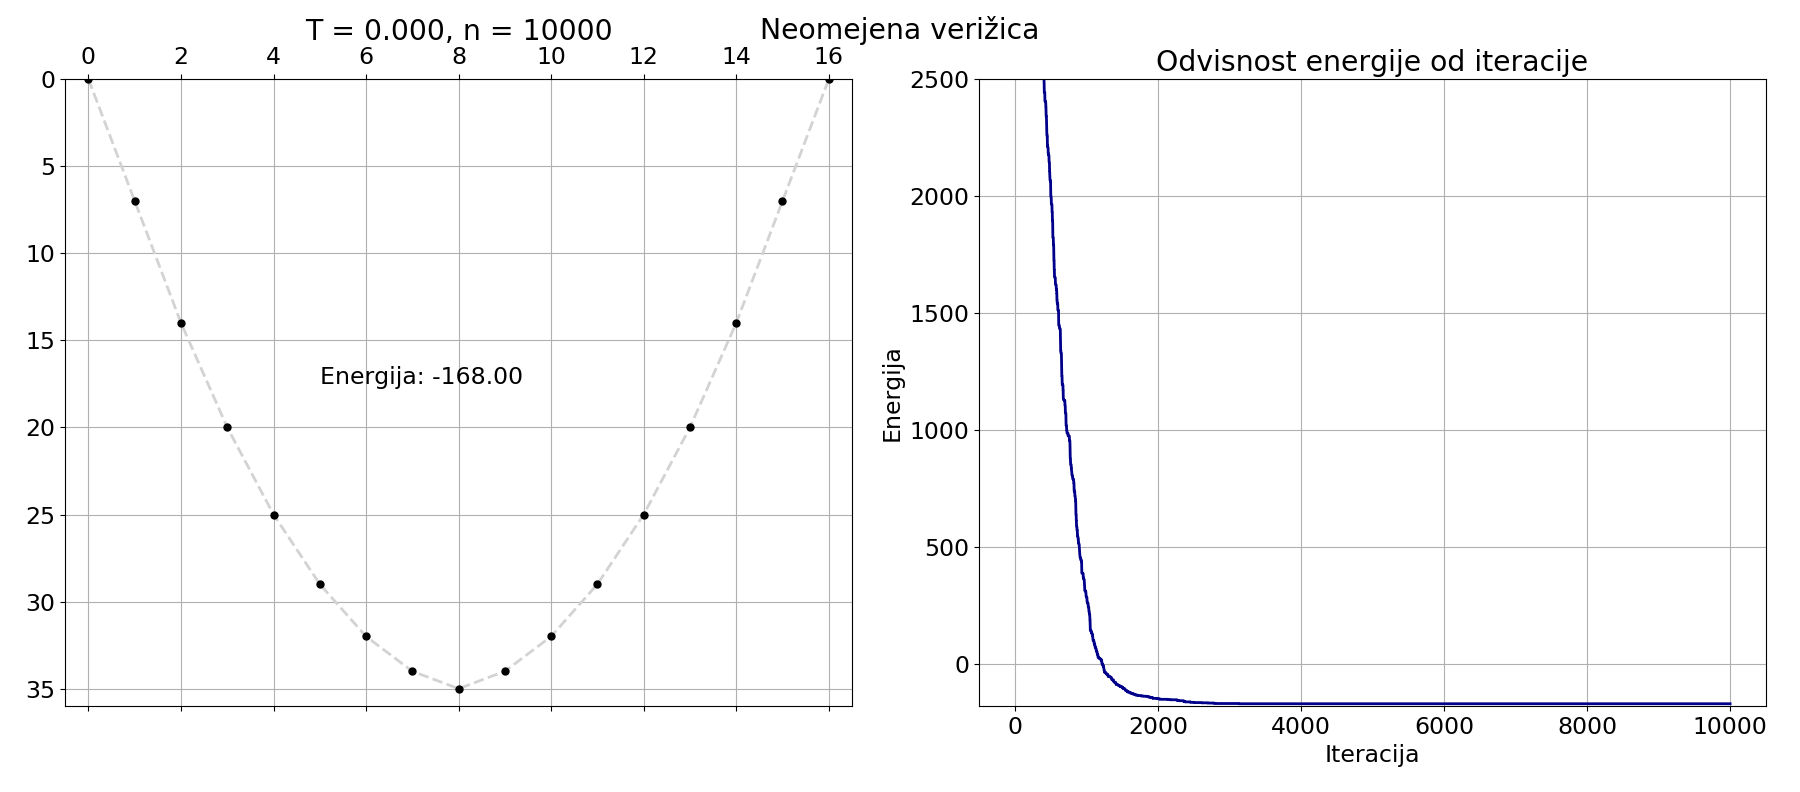
\includegraphics[width=16cm, height=4cm]{neomejena_globina_T0.png}

\end{figure} 
Pri neomejeni verižici vidimo podobno, fluktuacije so vse manjše, energija vedno manjša, in vse bolj se bližamo minimumu, ki je v tem primeru lokalni.
\subsection{Vpliv parametra $\alpha$ na sistem}
Parameter $\alpha = mg$ nam določa masa vsake molekule in gravitacijska sila. V praksi nam $\alpha$ pove kako velika je potencialna energija v primerjavi s prožnostno. Pričakujemo, da bo verižica bolj ugreznjena, saj nam dolžine niso več zelo pomembne.
\begin{figure}[H]

\centering
  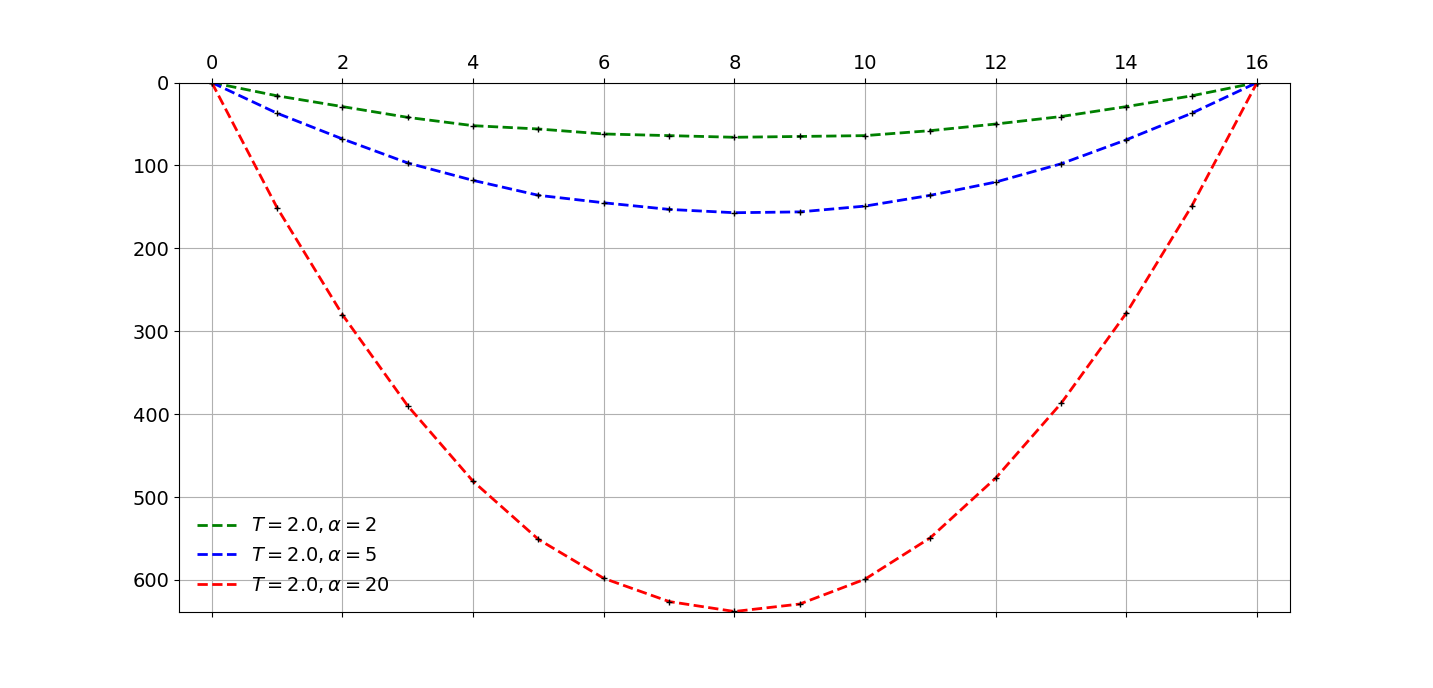
\includegraphics[width=10cm, height=4cm]{alfa.png}
\caption{Vpliv $\alpha$ nam zniža vrvico ker ima na minimizacijo veliko večji vpliv potencialna energija, kot razdalja med molekulami.}
\end{figure} 
\subsection{Energija verižice v odvisnosti od temperature }
Vzemimo dovolj iteracij ($n= 30000$), da bo zagotovo pretekel burn-in čas. Zanima kakašna je odvisnost \textbf{povprečja} minimuma energije vrvice od temperature. 
\begin{figure}[H]
\centering
  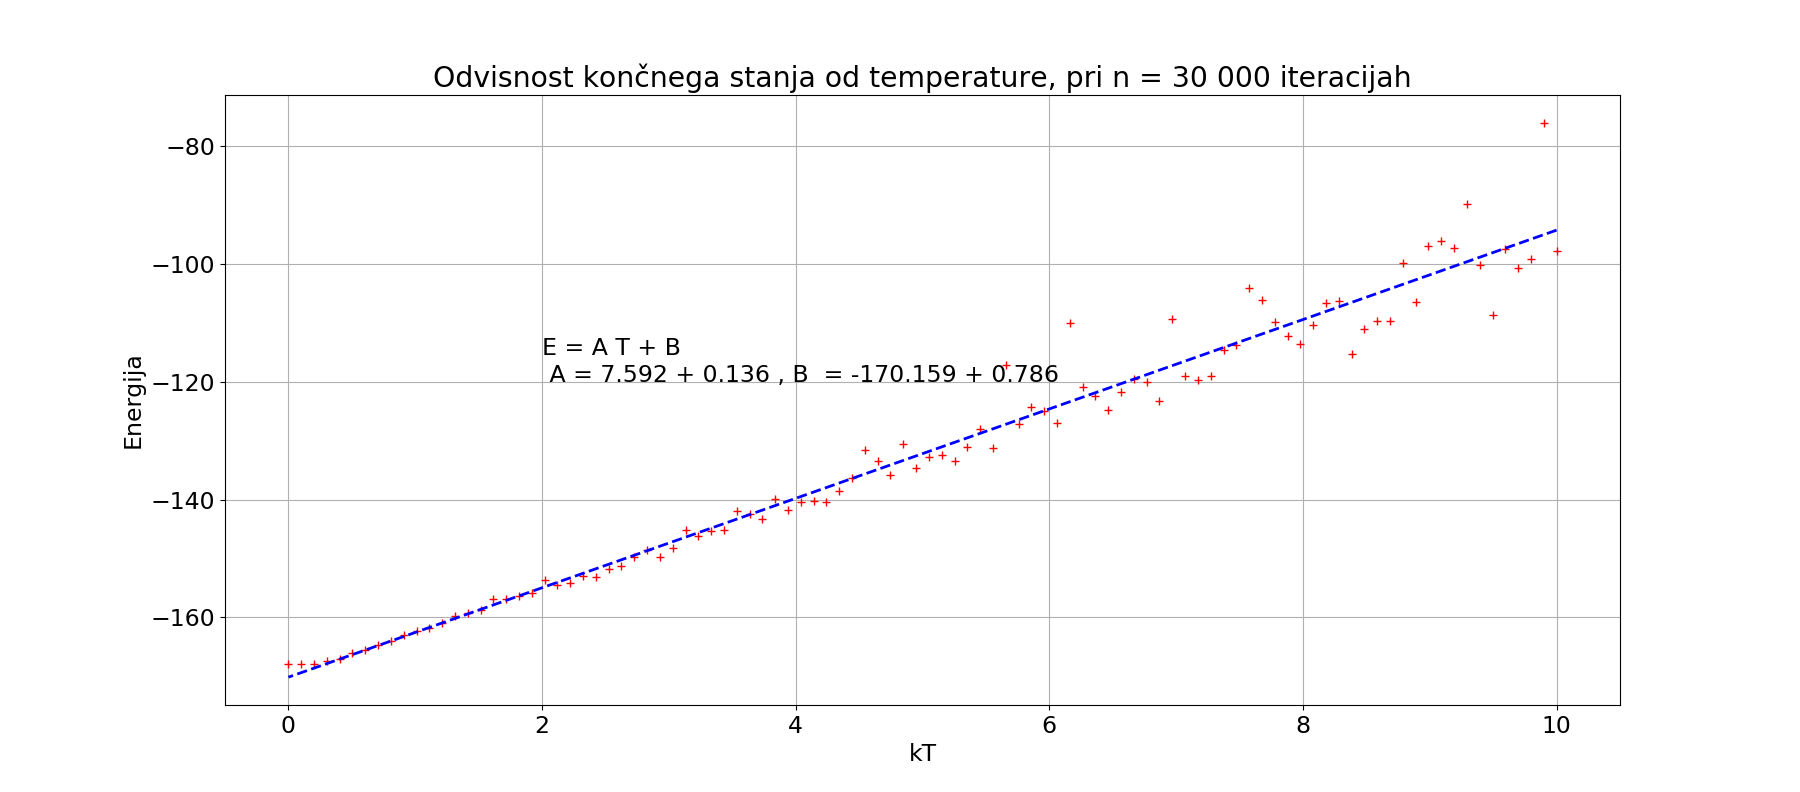
\includegraphics[width=16cm, height=6cm]{prva_energija.png}
\caption{Odvisnost energije stanja vrvice od temperature je linearna. Nižja kot je temperatura, bolj je vrvica v globalnem minimumu. Vidimo tudi, da s višanjem temperature energija vse bolj fluktuira, saj dopustimo prehod v manj verjetna stanja.}
\end{figure} 
\section{Izingov model}
Imamo 2D spinsko mrežo velikosti $N$, na katere naključno položimo spine v smeri gor in dol. Zapišimo energijo interakcij med spini
\begin{equation}
H = \sum_{i,j} -J_i S_i S_j - \sum_i H_i S_i 
\end{equation}
,kjer je $S_{i,j} = \pm 1$ in $i,j$ poteka med najbližjimi sosedi, saj je dlje interakcija zanemarljiva. Vzemimo $J_i = J$ in $H_i = H$ in tako zapišimo 
\begin{equation}
H =-J \sum_{i,j}  S_i S_j -H \sum_i  S_i 
\end{equation}
Spini so pri neki temperaturi v termalnem ravnovesju; torej se bodo iz začetnega premikali in obračali tako, da bo na koncu energija pri dani temperaturi energija minimalna oz. bo fluktuirala okoli.
\newline\newline
S metropolisovim algoritmom, dejansko ne bomo izvedli simuliranega ohlajanja, temveč le MCMC (Markov Chain Monte Carlo). Na vsakem koraku zapišemo verjetnost za sprejetje poteze kot 
\begin{equation}
 \frac{P(\vec{x'} \rightarrow \vec{x})} {P(\vec{x} \rightarrow \vec{x'})} = \frac{p(\vec{x')) g(vec{x}|x')}}{p(\vec{x})) g(vec{x'}|x)}
\end{equation}
g je v tem primeru verjetnost da izberemo stanje $x$ pri tem da smo imeli prej $x'$ in obratno, ki je v našem primeru kar $1 / N^2$ in se pokrajša, saj je za obe enaka. \newline\newline
\begin{wrapfigure}{r}{0.5\textwidth}
  \begin{center}
    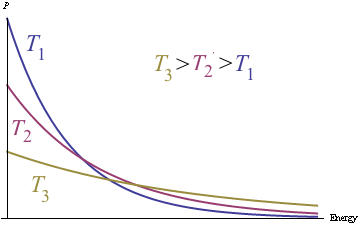
\includegraphics[width=0.48\textwidth]{Boltzmann.png}
  \end{center}
  \caption{}

\end{wrapfigure}
\newline\newline
Ker je v našem primeru željena porazdelitev Boltzmanova porazdelitev pri neki temperaturi - $P(\vec{x}) = Ae^{\frac{-E}{k_bT}}$, definirana za $E>0$ bomo preko naključnega sprehoda po večih iteracijah prišli v stacionarno stanje, kar pomeni, da bo vsako naslednje stanje porazdeljeno po boltzmanovi porazdelitvi, ki je tudi fizikalna porazdelitev statističnih sistemov po energijah. Pri nizkih temperaturah je ta porazdelitev vedno bolj strma in zato bo energija stanj vedno manj fluktuirala.
\newline\newline

\subsection{Stanja sistema pri različnih temperaturah}
Za začetek si poglejmo nekaj osnovnih ravnovesnih stanj pri različnih temperaturah pri mreži  velikosti 100x100.
 \begin{figure}[H]
\centering
  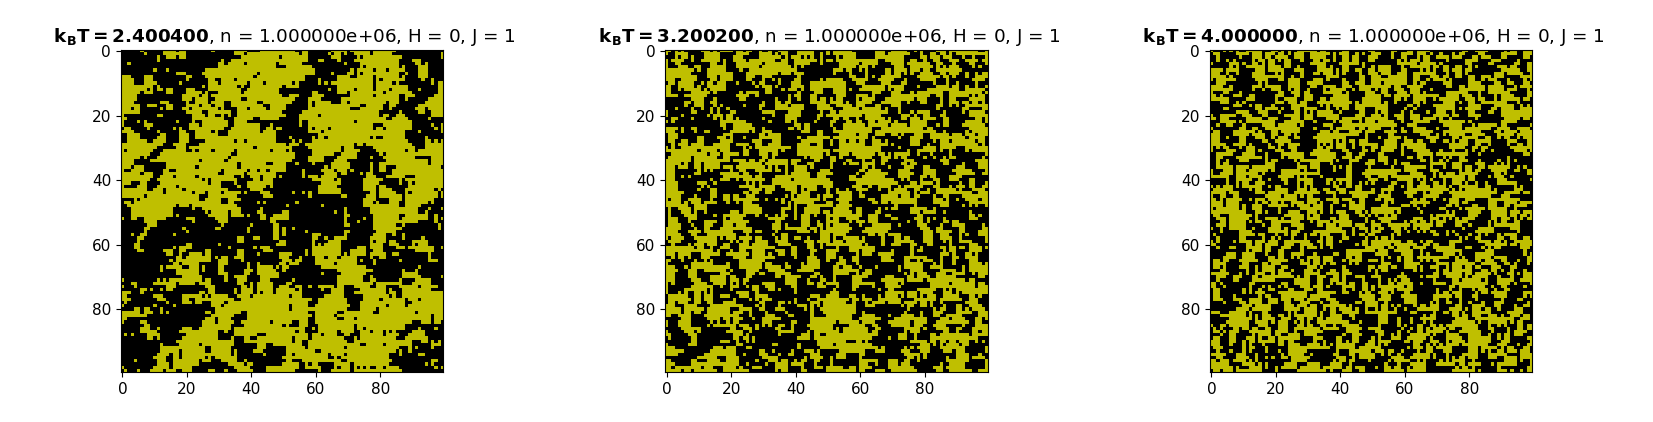
\includegraphics[width=17.5cm, height=5.5cm]{druga_domene2.png}

\end{figure}
 \begin{figure}[H]
\centering
  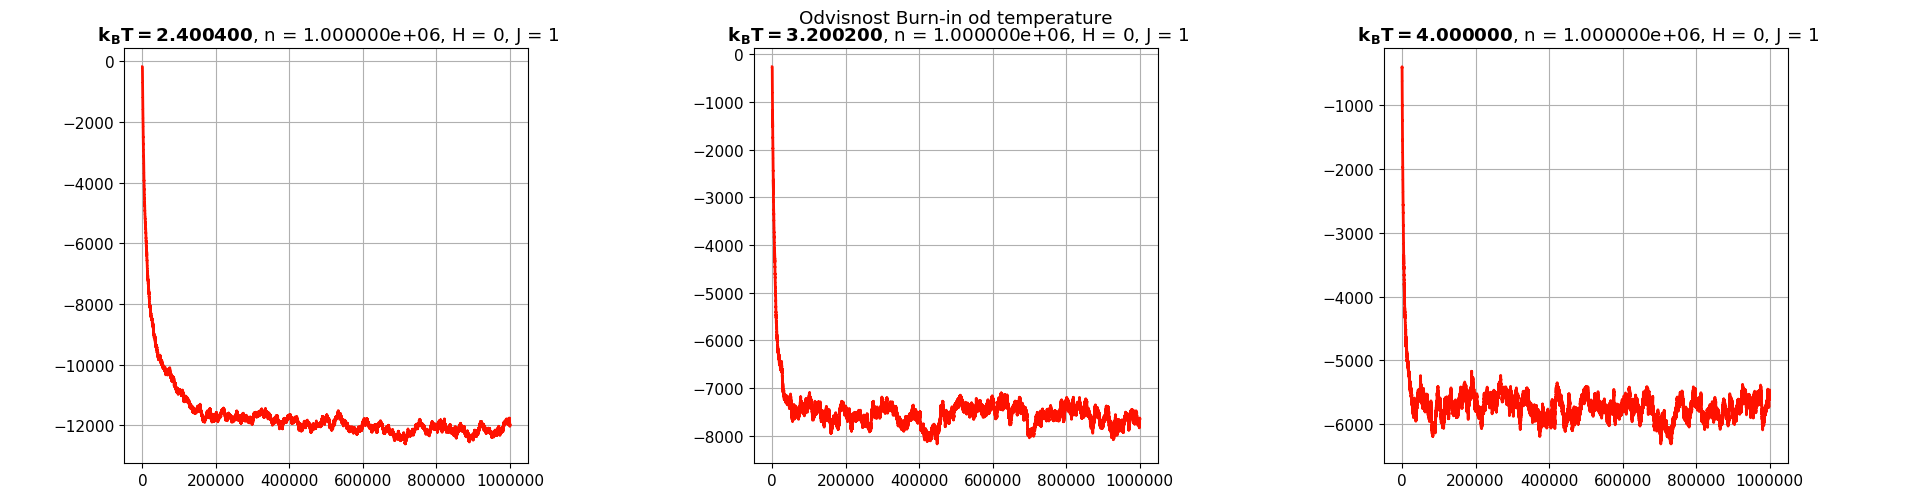
\includegraphics[width=17cm, height=5.5cm]{druga_domene2_burinin.png}
\caption{Prikaz stacionarnih stanj (od leve proti desni - 4 $k_B T$, 3.2 $k_BT$ , 2.4 $k_BT$). Vidimo, da se domene proti temperaturi $\frac{2}{k_BT}$ začenjajo vse bolj urejajti v otoke. Spodnja slika ima prikazan Burn-in fazo, opazimo tudi vedno manjšo velikost fluktuacij energije.}
\end{figure}  
 \begin{figure}[H]
\centering
\hspace{-1cm}
  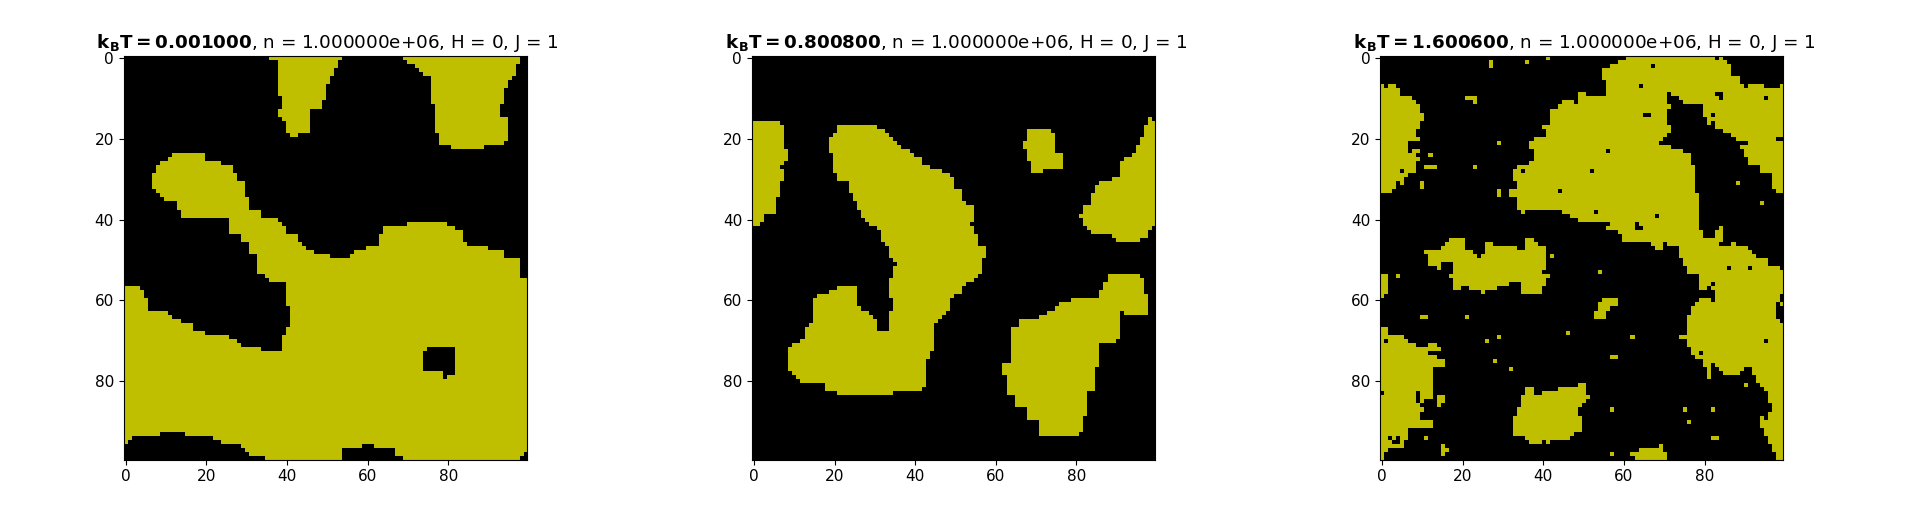
\includegraphics[width=18cm, height=5.5cm]{druga_domene1.png}
\caption{Prikaz stacionarnih stanj (pri manjši temperaturi od kritične se vzpostavijo domene, fluktuacije energije so manjše. Temperature si sledijo od $1.6$ do $0.001 k_BT$. }
\end{figure}
 \begin{figure}[H]
\centering
  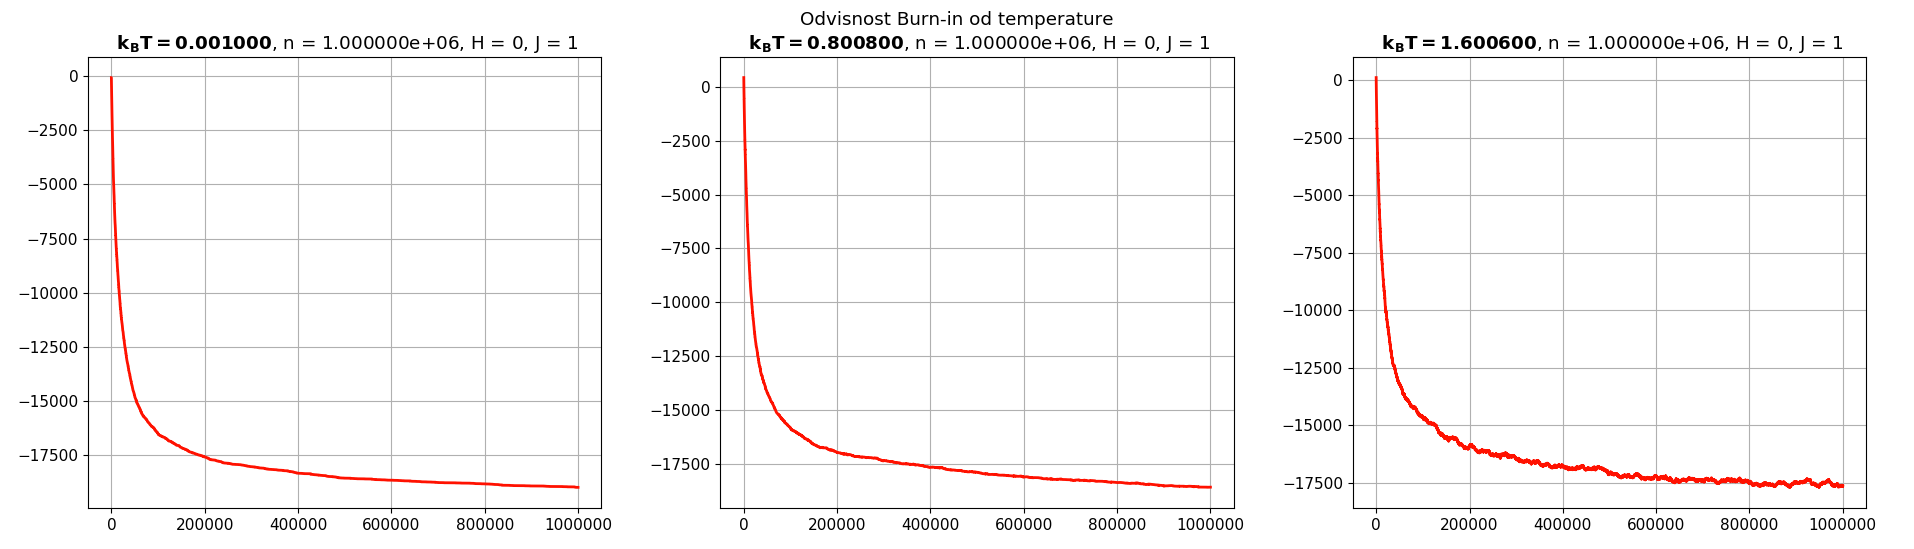
\includegraphics[width=17cm, height=5cm]{druga_domene1_burnin.png}

\end{figure}  
\subsection{Magnetizacija, energija, magnetna suscetibilnost v odvisnosti od temperature}
Ko enkrat preidemo burn-in fazo in začnemo naša stanja res vzorčiti po Boltzmanovi statistiki, lahko pustimo simulacijo da teče naprej in izračunamo povprečje energije, magnetizacije in z njimi povezane količine. Vzel sem $n = 3.000000e+07$ iteracij in po burn in fazi izračunal povprečno energijo in magnetizacijo za vsako temperaturo. Simulacija je trajala uro in pol.

 \begin{figure}[H]
\centering
  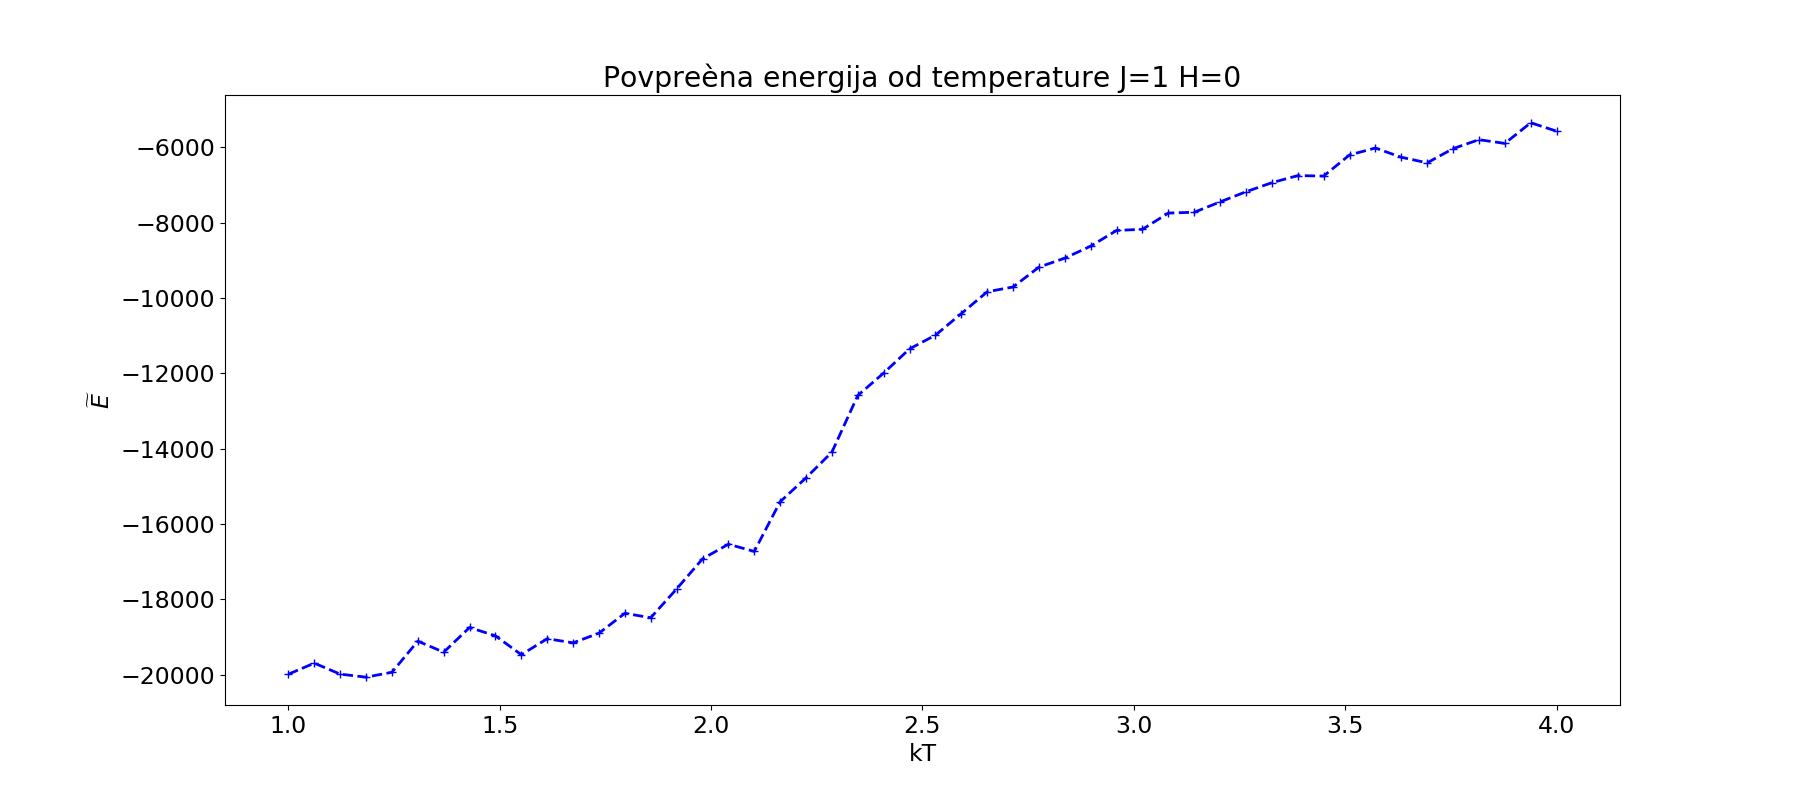
\includegraphics[width=17cm, height=5cm]{druga_energija.png}

\end{figure}  
 \begin{figure}[H]
\centering
  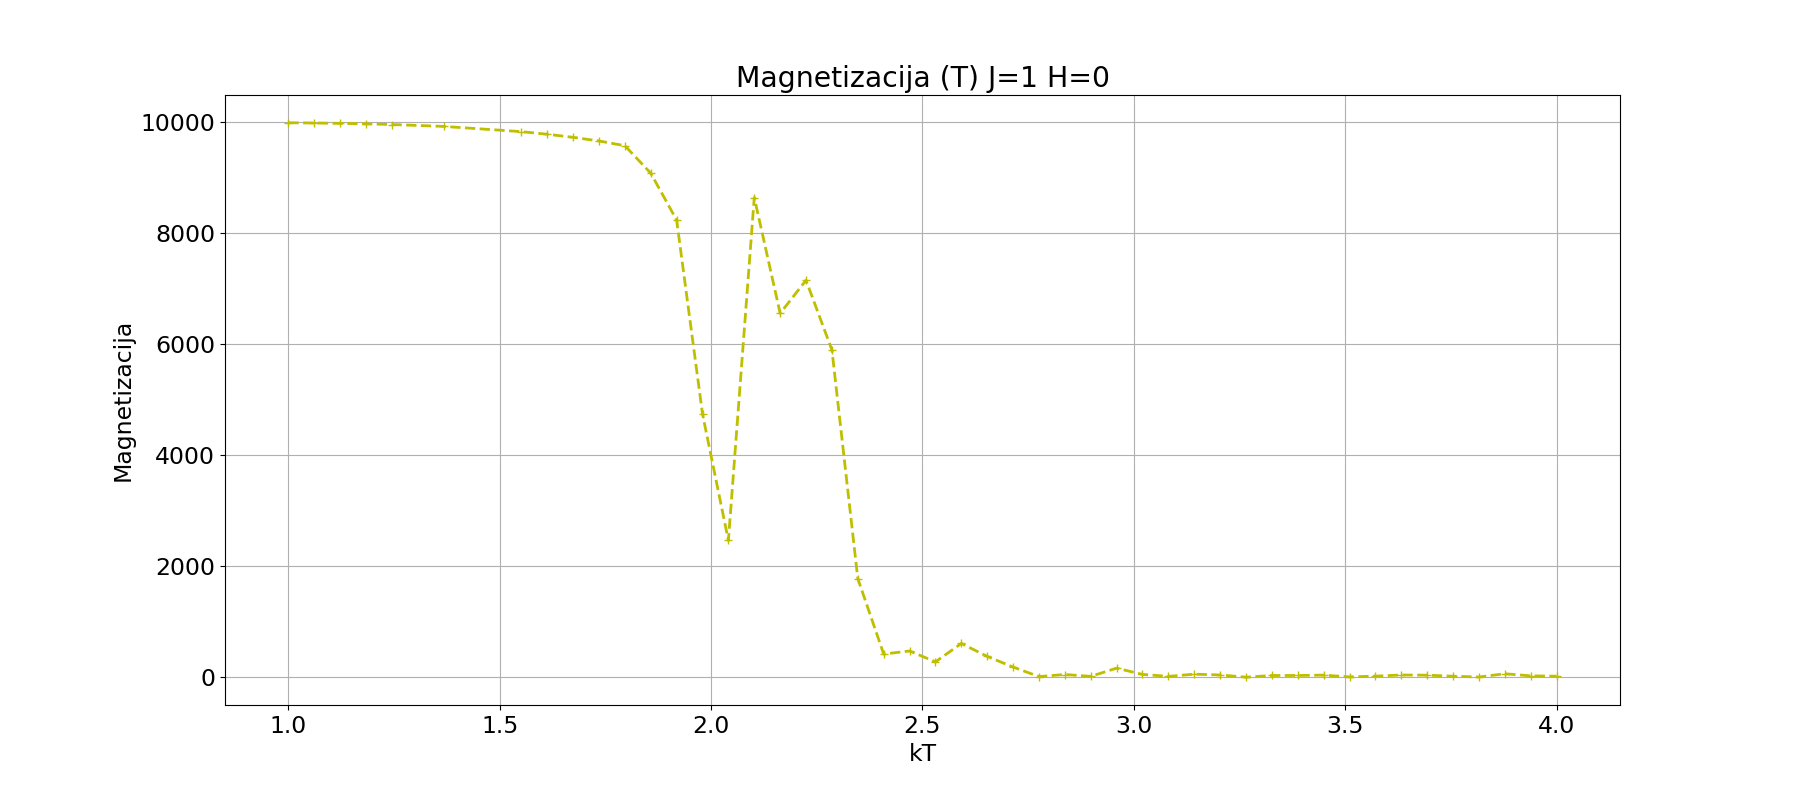
\includegraphics[width=17cm, height=5cm]{druga_magnetizacija.png}
\caption{Odvisnost magnetizacije od temperature nam pokaže fazni prehod pri temperaturi $k_B T_c/J = \frac{2}{\ln(1+\sqrt{2})} \approx 2.26918531421$}

\end{figure}  
 \begin{figure}[H]
\centering
  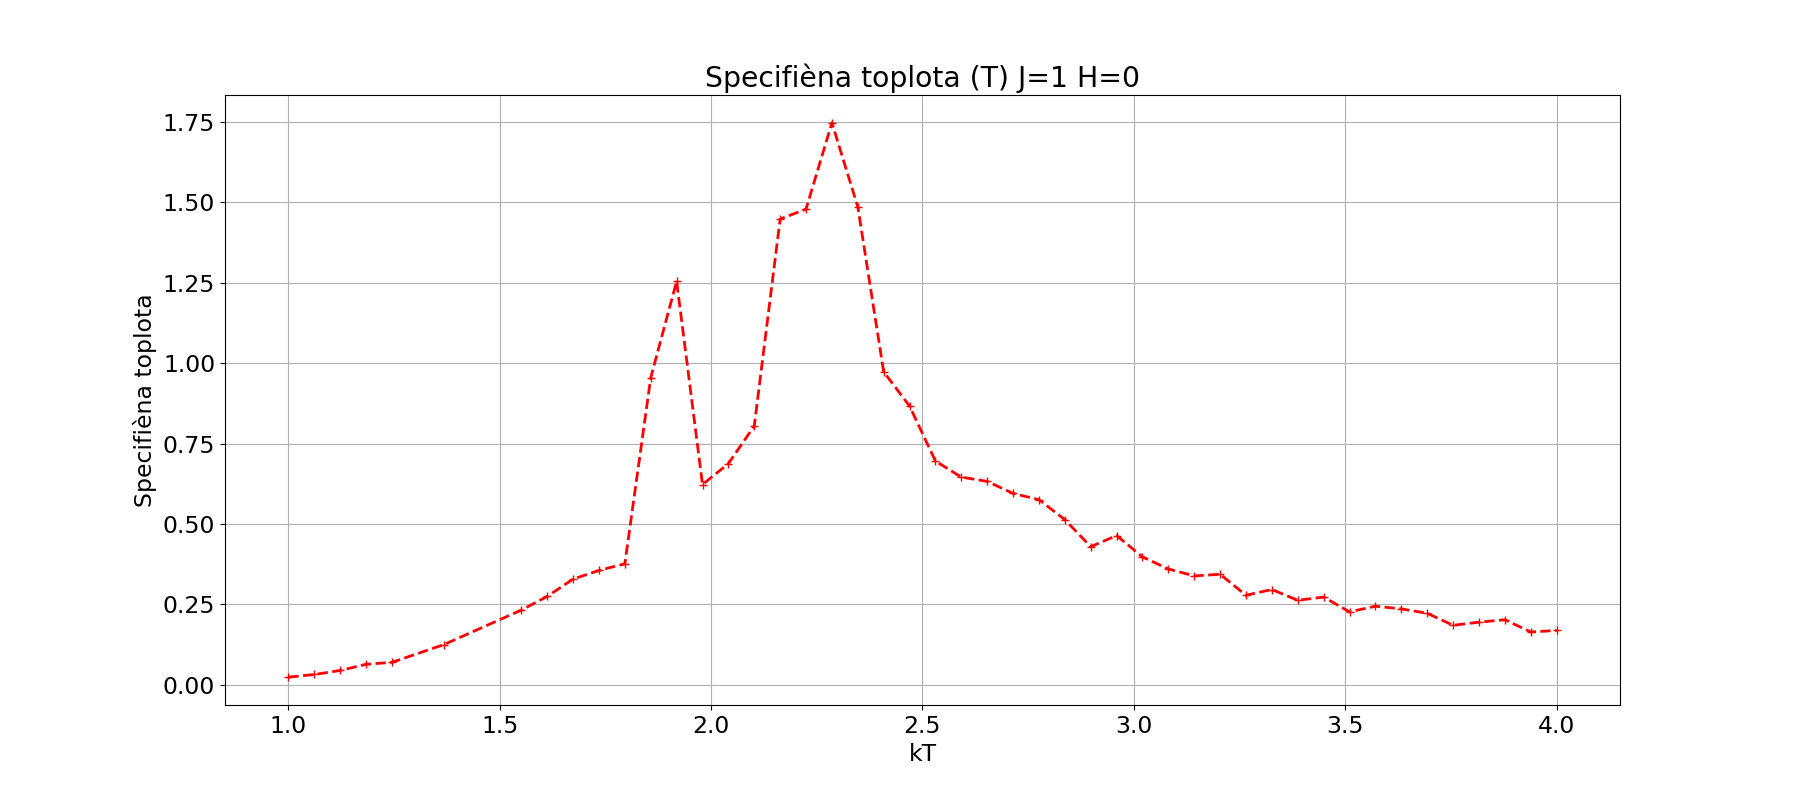
\includegraphics[width=17cm, height=5cm]{specificna_toplota.png}
\caption{Vidimo, da v bližini kritične temperature naraste specifična toplota, ki na to ne pade več na 0 amapk ostane konstantna}

\end{figure}  
 \begin{figure}[H]
\centering
  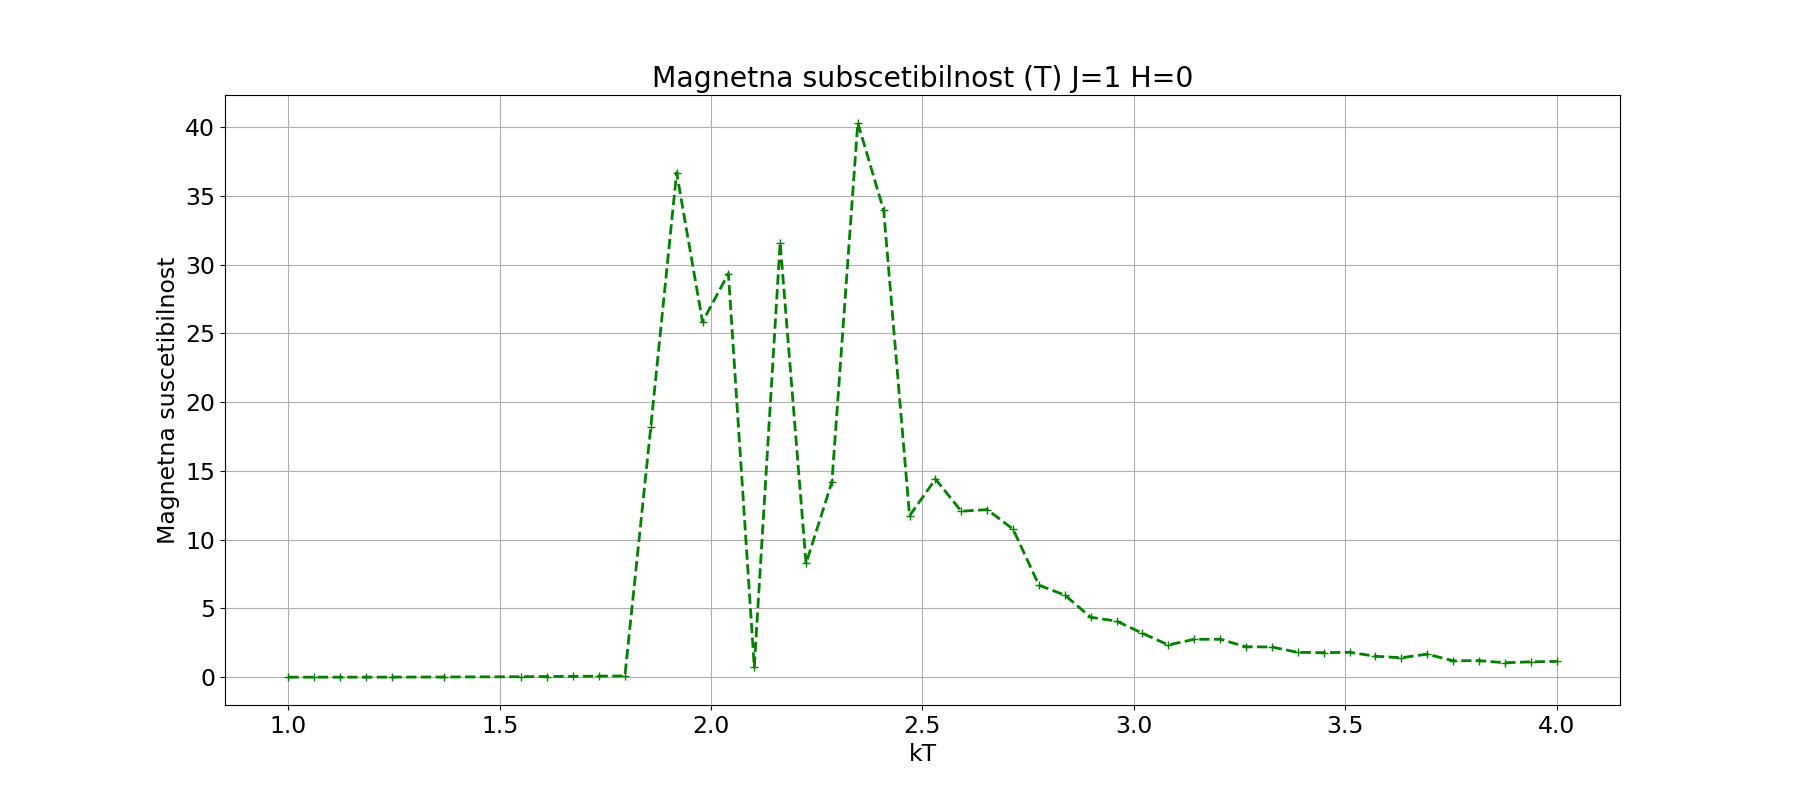
\includegraphics[width=17cm, height=5cm]{subscetiblnost.png}
\caption{Vidimo, da po faznem prehodu magnetna subscetibilnsot pade na 0.}

\end{figure} 

\section{Simulirano ohlajanje - optimizacija trgovskega potnika}
Oglejmo si sedaj optimizacijski problem. Imamo mrežo mest (lahko je simetrična npr. kvadratna, ali pa poljubna), na katerega postavimo $N$ točk, ki jih mora trgovski potnik obiskati. Zanima nas kakšna je najkrajša pot trgovskega potnika, da bo pot sklenjena od začetka do konca. Pot bo najkrajša, ko bo pot $S$ najkrajša 
\begin{equation}
S = \sum_i^n \sqrt{(x_i -x_{i+1})^2 + (y_i -y_{i+1})^2)} = min
\end{equation}
Za energijo tako lahko vzamemo $S$ in uporabimo simulirano ohljanje. Implementiral bom problem s začetno kvadratno mrežo in na njej enakomerno porazdeljena mesta, čeprav se lahko mesta nahajajo na poljubni točki. Za začetni približek vzamemo naključni vrstni red mest $[0,1,2,...,L]$, kjer je $L$ število mest.\newline\newline
Vsako potezo naključno izberemo dva para, ki ju zamenjamo. Izbrati si je treba tudi plan hlajenja. Sam se prilagojeval glede na velikost problema. 
Začel sm s $N =36$ mesti, kjer je bilo dovolj 6 stopenjsko ohlajanje po $10^4$ iteracij, in je temperatura padala enakomerno $T = 10,..,0.1$.\newline\newline S višanjem števila mest smo morali za optimizacijo stopnje ohlajanja zviševati. Število stopenj je bilo potrebno najti za vsako dimenzijo posebaj s poskušanjem.
  
 \begin{figure}[H]
\centering
  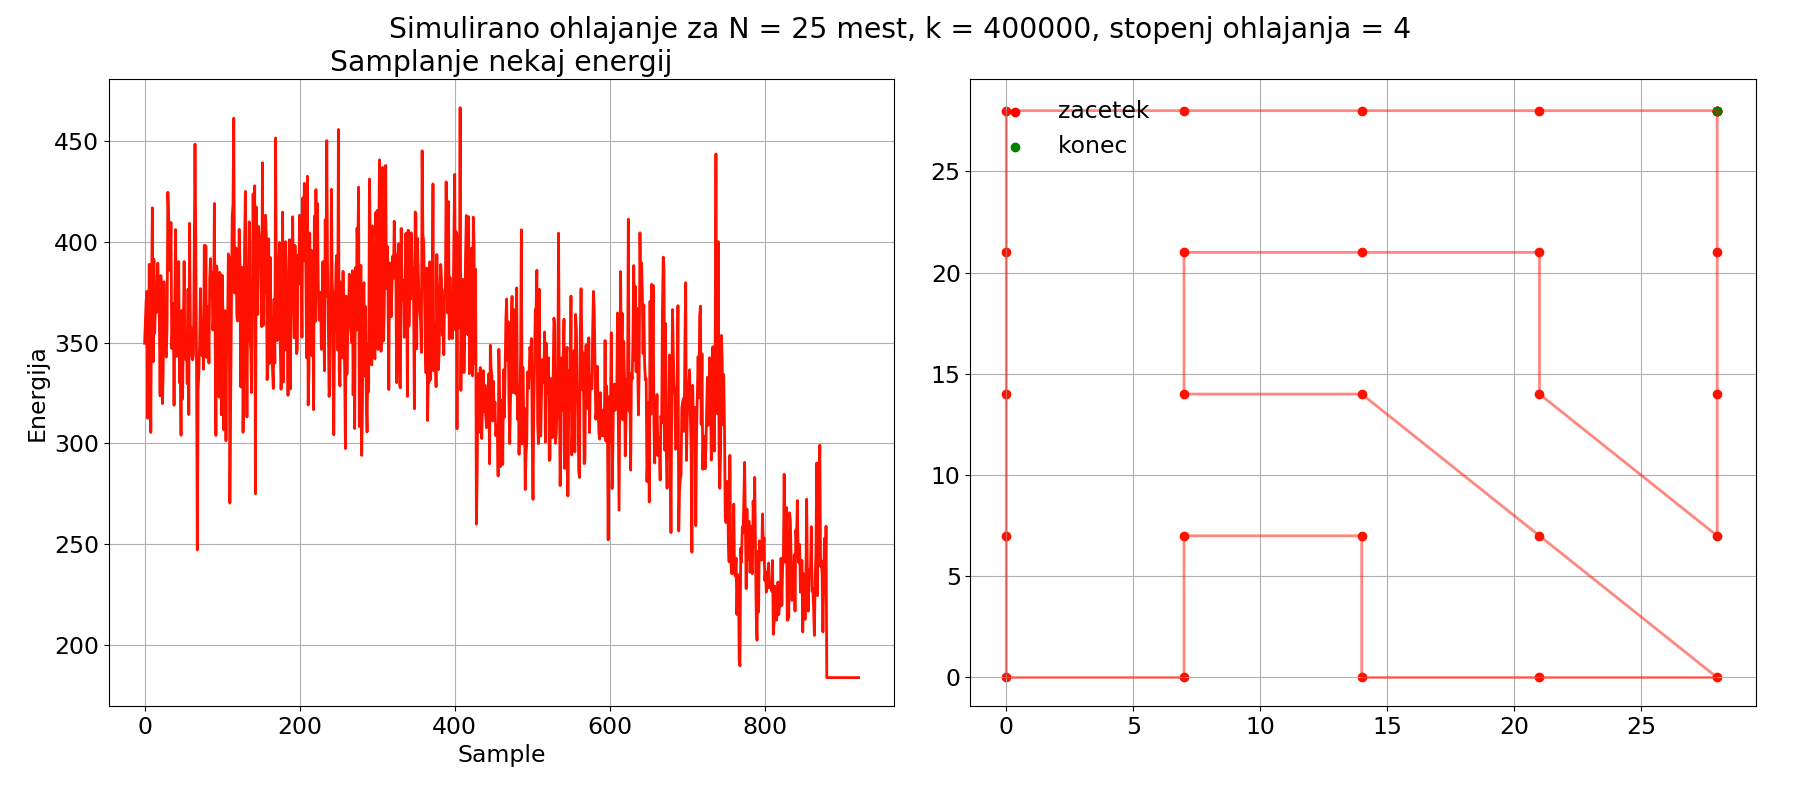
\includegraphics[width=17cm, height=5cm]{tretja_N25.png}
\caption{Rešitev za 25 mest.}
\end{figure} 

 \begin{figure}[H]
\centering
  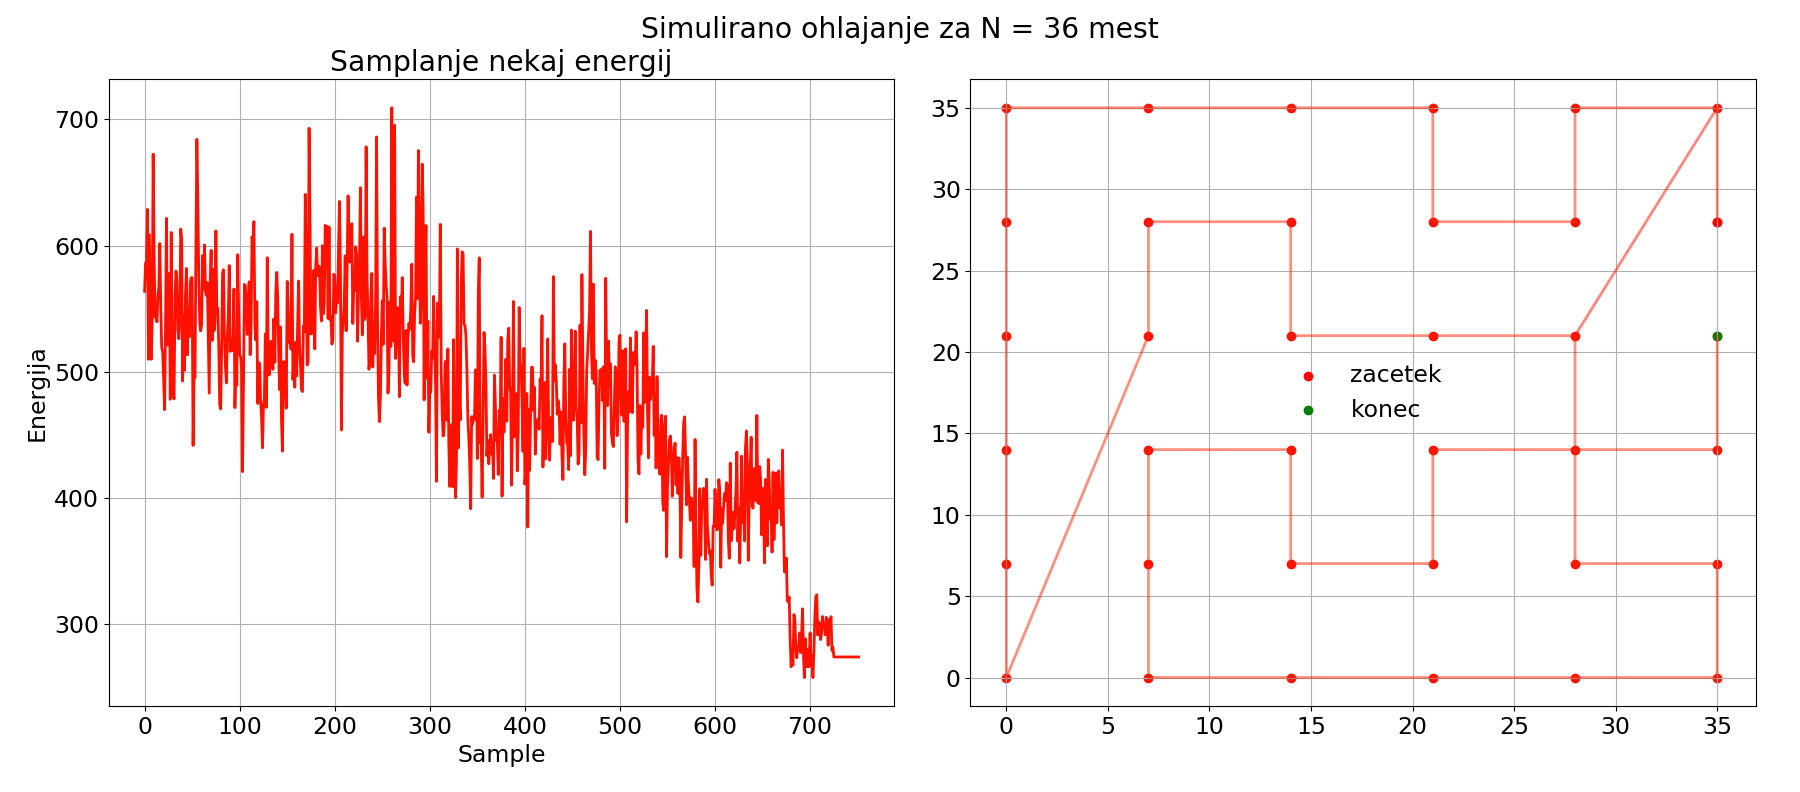
\includegraphics[width=17cm, height=5cm]{tretja_N36.png}
\caption{Rešitev za 36 mest.}
\end{figure} 
  \begin{figure}[H]
\centering
  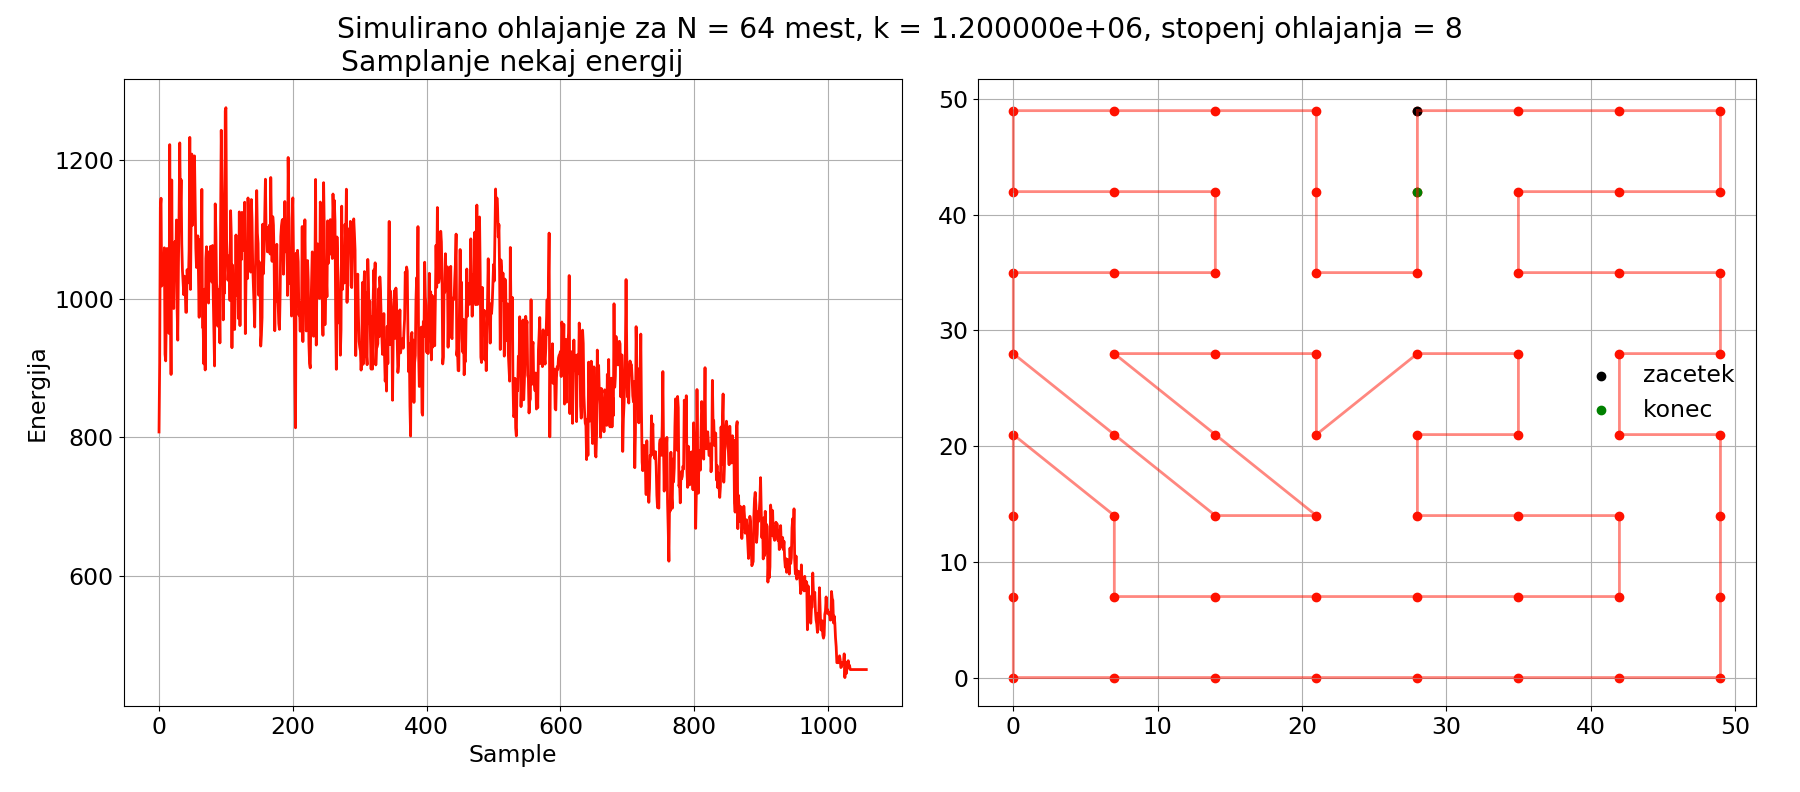
\includegraphics[width=17cm, height=5cm]{tretja_N64.png}
\caption{Rešitev za 64 mest. Simulacija traja pol minute. časovna zahtevnost pa je eksponentna.}


\end{figure} 
Ugotovimo da univerzalnega recepta za plan ohlajanja ni, preprosto potrebno je zelo optimizirano spisati program in nato poskusiti najti optimalno rešitev. Če analtične rešitve ne poznamo je potrebno večkrat posimulirati in pogledati kaj se dogaja s energijo, saj smo le tako lahko prepričani, da bomo padli v globalni minimum.\newline\newline
Ppomnimo, da bi s novimi pogoji na mestih (denar, ki ga lahko v mestu pridobimo),  naravne ovire (reka, kanjon,..), močno povečajo časovno zahtevnost simulacije. 
\section{Zaključek}
Naučili smo se kaj je so Markovske verige in kako jih izkorišča Metropolis Hasting algoritem za pridobivanje vzorcev iz več dimenzionalnih porazdelitev (npr. pri isingu $N = 500*500$), prek tega, da naključne procese usmerjamo v smeri naše porazdelitve, a še vseeno pogledamo tudi naokoli po faznem prostoru. Pogledali smo si tudi algoritem simuliranega ohlajanja in ugotovili, da je potrebno izbrati plan ohlajanja in paziti na optimalni zapis kode, saj so optimizacije te vrste lahko zelo počasne. 

\end{document}